%=======================================================================
%  Intercept: Chase-and-Intercept Routing for Metro Vancouver Transit
%  IEEE conference paper (IEEEtran). Compiles on Overleaf out of the box.
%  Build: pdfLaTeX  ->  BibTeX  ->  pdfLaTeX  ->  pdfLaTeX
%=======================================================================
\documentclass[conference]{IEEEtran}
\IEEEoverridecommandlockouts

\usepackage{cite}
\usepackage{amsmath,amssymb,amsfonts}
\usepackage{algorithmic}
\usepackage{graphicx}
\usepackage{textcomp}
\usepackage{xcolor}
\usepackage{booktabs}
\usepackage{url}
\usepackage{pgfplots}
\pgfplotsset{compat=1.17}
\usepackage[hidelinks]{hyperref}

\def\BibTeX{{\rm B\kern-.05em{\sc i\kern-.025em b}\kern-.08em T\kern-.1667em\lower.7ex\hbox{E}\kern-.125emX}}

\begin{document}

\title{Intercept Routing for Public Transit:\\ Boarding Connections via High-Frequency Services}

\author{\IEEEauthorblockN{Pratik Bashyal}
\IEEEauthorblockA{\textit{Department of Computer Science} \\
\textit{Fairleigh Dickinson University}\\
Vancouver, BC, Canada \\
bashyalpratik26@gmail.com}}

\maketitle

\begin{abstract}
Conventional transit trip planners (Google Maps, the Transit app, agency apps)
optimize an itinerary under the implicit assumption that a rider boards the
chosen route at the stop nearest the origin. This assumption silently discards a
class of itineraries that experienced riders use intuitively: riding a
\emph{high-frequency connector} to a \emph{downstream junction} on a target
route and boarding the target vehicle there---catching a bus the rider would
otherwise miss while walking to the nearest stop. We call this
\emph{chase-and-intercept} routing. We formalize the intercept structure,
implement a dependency-free planner over the live Metro Vancouver (TransLink)
feed---239 routes, 8{,}916 stops, and 1.84~million stop-time events---and
automatically detect intercept junctions with no hand-coding. On a reproducible
sample of 1{,}500 transit-servable origin--destination (O--D) pairs during the
morning peak, a direct single-route itinerary exists for only 13.2\% of pairs,
whereas an intercept structure exists for 57.3\%. Crucially, when a direct
route \emph{does} exist, a more-frequent connector to a downstream junction is
\emph{also} available 43.4\% of the time, with a median connector-to-target
frequency advantage of $3.1\times$ (median target headway 17.9~min vs.\ connector
6.0~min). A simple headway-based reliability model shows the intercept reduces
expected boarding wait by 66\% in these cases. We corroborate the structural
findings with a real, lived trip in East Vancouver. The results indicate that
intercept routing is common, mechanically well-defined, and best realized with
real-time vehicle positions; we release the planner and evaluation harness as an
open prototype.
\end{abstract}

\begin{IEEEkeywords}
public transit, trip planning, journey planning, GTFS, real-time, routing
algorithms, Metro Vancouver, reliability
\end{IEEEkeywords}

%=======================================================================
\section{Introduction}
%=======================================================================
Public-transit trip planners have converged on a familiar interaction model: the
rider enters an origin and destination, and the planner returns a small set of
itineraries ranked by arrival time, number of transfers, and walking distance.
Behind this interface, modern planners solve a well-studied earliest-arrival or
Pareto-optimal journey problem over a timetable
graph~\cite{raptor,csa,transferpatterns}. These systems are fast, correct, and
widely used.

Yet riders in the field routinely perform a maneuver that mainstream planners do
not surface. Consider a rider near a major arterial who wants to board an
infrequent cross-town route. The planner directs them to walk to that route's
nearest stop. But by the time the rider arrives on foot, the target bus---which
was already in motion---has passed. An experienced rider instead boards a
\emph{different}, high-frequency route going the same general direction, rides it
to a \emph{downstream} point where the two routes meet, and boards the
\emph{same} target vehicle there. The frequent connector acts as a faster
``carrier'' to a junction the target has not yet reached.

We call this \textbf{chase-and-intercept} routing. It is not a shortcut in
graph-distance terms---on a static timetable it often ties the direct
itinerary---but it is a decisive improvement in \emph{reliability} and in the
real-time ability to \emph{catch a specific moving vehicle}. Standard planners
discard it precisely because it looks like ``an extra transfer for no scheduled
time savings,'' so their ranking heuristics prune it.

This paper makes the following contributions:
\begin{itemize}
  \item We \textbf{formalize} the chase-and-intercept structure and distinguish a
  \emph{genuine} intercept (a more-frequent connector reaching a junction
  downstream of where the rider could have boarded directly) from an ordinary
  two-leg transfer (Section~\ref{sec:problem}).
  \item We build a \textbf{dependency-free prototype} (Node.js + SQLite) that
  loads the full live TransLink GTFS feed and \textbf{automatically detects
  intercept junctions} with no per-route hand-coding, together with a RAPTOR-lite
  multi-leg search and a real-time (GTFS-RT) rescue evaluator
  (Section~\ref{sec:system}).
  \item We provide a \textbf{reproducible quantitative evaluation} over 1{,}500
  sampled O--D pairs showing that intercept opportunities are common and
  measurably improve expected waiting time, plus a two-seed robustness check
  (Section~\ref{sec:eval}).
  \item We corroborate the analysis with a \textbf{validated real-world case
  study} in East Vancouver and discuss why the headline feature fundamentally
  requires real-time data (Sections~\ref{sec:eval} and~\ref{sec:discussion}).
\end{itemize}

%=======================================================================
\section{Related Work}
%=======================================================================
\textbf{Journey planning algorithms.} Earliest-arrival and multi-criteria
journey planning on timetables is mature. RAPTOR~\cite{raptor} organizes the
search into rounds, each adding one additional trip, and is naturally suited to
bounding the number of transfers. The Connection Scan Algorithm~\cite{csa}
reduces routing to a single linear scan over time-sorted connections. Transfer
Patterns~\cite{transferpatterns} precompute the small set of optimal transfer
sequences to answer continental-scale queries in milliseconds. Our prototype uses
a RAPTOR-style round-based search (Section~\ref{sec:system}) but differs in
\emph{objective}: rather than ranking solely by arrival time and transfer count,
we explicitly surface intercept itineraries that these objectives would prune.

\textbf{Production planners.} General-purpose engines such as
OpenTripPlanner~\cite{otp} and the planners inside consumer apps produce
Pareto-optimal itineraries over GTFS~\cite{gtfs} and, increasingly,
GTFS-Realtime~\cite{gtfsrt}. These systems do consider transfers, but their
ranking penalizes additional boardings and they assume boarding at the nearest
stop of each route. The intercept maneuver is thus systematically
down-ranked or omitted. Our contribution is complementary: an
\emph{intercept-aware ranking layer} that can sit on top of such an engine.

\textbf{Frequency and reliability.} The waiting-time consequences of service
frequency are classical. For uniformly random passenger arrivals the expected
wait is half the headway; with headway variance it is larger, a result tracing to
Welding~\cite{welding1957} and formalized in urban operations
research~\cite{osuna1972,larson1981}. Our reliability model
(Section~\ref{sec:eval}) applies these results to quantify why riding a frequent
connector to a junction is more robust than waiting for an infrequent target.

%=======================================================================
\section{Problem Formulation}
\label{sec:problem}
%=======================================================================
\subsection{Timetable model}
Let the transit network be a set of stops $S$, routes $R$, and trips $T$. Each
trip $\tau \in T$ belongs to a route $r(\tau)\in R$ and visits an ordered
sequence of stops $\langle s_1^{\tau}, s_2^{\tau}, \ldots \rangle$ with scheduled
departure times $d^{\tau}(s_i)$. A service calendar maps each trip to the dates
on which it operates. For a stop $s$ and route $r$ within a time window
$[w_0, w_1]$, the \emph{headway} $h(r,s)$ is the median gap between consecutive
scheduled departures of $r$ at $s$.

\subsection{Direct boarding (the baseline)}
Given an origin $o$ and destination $g$ (both as geographic points), a route
$r$ is a \emph{target} if some stop of $r$ lies within a destination radius
$\rho_g$ of $g$. For a target $r$, the \emph{direct boarding stop}
$b^\star(r)$ is the stop of $r$ nearest to $o$ within an origin radius $\rho_o$.
If such a stop exists and precedes the destination stop along the route, the trip
is \emph{directly boardable}---this is the itinerary mainstream planners return.

\subsection{The intercept structure}
A \emph{connector} is any route $c \neq r$ that serves a stop within $\rho_o$ of
the origin. Let $\langle s_1^r,\dots,s_m^r\rangle$ be a representative trip of the
target $r$, with the destination stop at position $p_g$ and the direct boarding
stop (if any) at position $p_b$. A stop $s_j^r$ with $p_b < j \le p_g$ is an
\emph{intercept junction} for connector $c$ if some stop of $c$ lies within a
junction radius $\rho_J$ of $s_j^r$. Intuitively: the rider boards $c$ near the
origin, rides it to the junction $s_j^r$---which is \emph{downstream} of where
they could have boarded $r$ directly---and boards $r$ there.

We call the structure a \textbf{genuine intercept} when two conditions hold:
\begin{enumerate}
  \item the target is directly boardable (so a na\"ive planner would simply tell
  the rider to walk to $b^\star(r)$); and
  \item the connector is substantially more frequent than the target at the
  relevant stops, i.e.\ the \emph{frequency advantage}
  \begin{equation}
    \alpha \;=\; \frac{h(r, s_j^r)}{h(c, b^\star(c))} \;\ge\; \alpha_{\min},
    \label{eq:adv}
  \end{equation}
  where $b^\star(c)$ is the connector's boarding stop near the origin. We use
  $\alpha_{\min}=1.5$.
\end{enumerate}
Condition~(1) ensures we are not merely describing an ordinary transfer that a
rider would take because no direct route exists; condition~(2) captures the
mechanism that makes the maneuver worthwhile---the connector arrives often enough
that the rider is far less exposed to just-missing the target.

\subsection{Why schedule time alone understates the value}
On a static timetable, boarding $r$ at $b^\star(r)$ and boarding the \emph{same}
vehicle of $r$ at the downstream junction $s_j^r$ yield identical arrival times:
it is one vehicle. The intercept's value is therefore not scheduled travel time
but \emph{reliability and realizability}: (i) the frequent connector reduces the
chance the rider mistimes the single infrequent target, and (ii) with real-time
positions, the connector can catch a target the rider provably cannot reach on
foot. We quantify (i) analytically in Section~\ref{sec:eval} and demonstrate (ii)
in the case study.

%=======================================================================
\section{System Design}
\label{sec:system}
%=======================================================================
\subsection{Overview}
\emph{Intercept} is a dependency-free web application. The backend is Node.js
with a single native dependency, \texttt{better-sqlite3}~\cite{bettersqlite};
the frontend is a Google-Maps-style Leaflet~\cite{leaflet} interface. There is no
heavyweight routing engine; the intercept logic is implemented directly so the
structure is transparent and auditable.

\subsection{Data ingestion}
We load the complete TransLink static GTFS feed~\cite{translink,gtfs} into SQLite:
routes, stops, trips, stop\_times, calendar, calendar\_dates, and shapes. The
loaded feed contains 239 routes, 8{,}916 geolocated stops, and 1.84~million
stop-time events. Live data uses the GTFS-Realtime v3
endpoints~\cite{gtfsrt}: vehicle positions and trip updates (predicted arrivals),
decoded from Protocol Buffers.

\subsection{Automatic junction detection}
A key design goal was that intercept junctions must be \emph{discovered}, not
configured. For a target route we take its representative (longest active) trip
and, for every stop, query a spatial grid for nearby stops of candidate
connector routes within $\rho_J$. Buckets of $\approx 0.004^{\circ}$
($\sim$300--440~m) make neighbor lookups $O(1)$ in practice. The detector
reproduces, with zero hand-coding, the real junction used in our case study:
the \#26 stop \emph{``Rupert St @ E 41 Ave''} and the \#41/R4 stop
\emph{``E 41 Ave @ Rupert St''}, 63~m apart.

\subsection{Multi-leg search}
Journey planning uses a RAPTOR-lite round-based search~\cite{raptor} with up to
two vehicle legs plus foot transfers. Round~0 seeds all stops walkable from the
origin; each subsequent round boards the earliest reachable trip per
route--direction and relaxes short foot transfers (within $\rho_T=250$~m) to reach
nearby stops---exactly the hop that realizes a junction transfer. Per-round
earliest-arrival labels let us reconstruct and compare \emph{direct} versus
\emph{intercept} itineraries for the same O--D pair.

\subsection{Real-time rescue evaluation}
The live module takes each currently moving vehicle of a target route and decides
whether the rider can catch it by \emph{walking} to the direct stop versus by
taking a \emph{connector} to a downstream junction, using predicted arrival
times. It emits a \textsc{rescue} verdict when the rider would miss the vehicle on
foot but the connector catches it---precisely the maneuver this paper studies.

\subsection{Parameters}
Unless noted, we use walking speed $1.3$~m/s, origin/destination radii
$\rho_o=\rho_g=500$~m, junction radius $\rho_J=200$~m, transfer radius
$\rho_T=250$~m, and a board buffer of 60~s. These are deliberately conservative
and match the values in the released code.

%=======================================================================
\section{Evaluation}
\label{sec:eval}
%=======================================================================
We ask three empirical questions: (Q1) \emph{How common} are intercept
structures? (Q2) \emph{How large} is the frequency advantage they offer? (Q3)
\emph{How much} do they improve boarding reliability? We answer all three with a
reproducible batch experiment over the real feed, then ground them in a lived
trip.

\subsection{Experimental setup}
We sample O--D pairs by drawing random pairs of stops whose straight-line
separation is between 1.5 and 9~km (a realistic urban-trip range), using a seeded
pseudo-random generator for reproducibility. A pair is \emph{transit-servable} if
stops exist within $\rho_o$ of the origin and $\rho_g$ of the destination. All
headways are computed on a representative weekday (Wednesday, 2026-10-07) in the
morning peak window $[\,07\!:\!00,\,10\!:\!00\,]$, using only services active on
that date per the GTFS calendar. The primary run uses $N=1500$ pairs (seed~42);
we repeat with seed~7 to check stability. The entire batch runs in under two
seconds on a laptop.

\subsection{Q1: Prevalence of intercept structures}
Table~\ref{tab:prev} and Fig.~\ref{fig:prev} summarize prevalence. Only 13.2\% of
servable pairs have a \emph{direct} single-route itinerary of the kind
mainstream planners prefer, confirming that most real trips already require a
transfer. An \emph{intercept structure}---a connector from the origin reaching a
downstream junction on a destination-serving route---exists for 57.3\% of pairs.
A \emph{genuine} intercept (direct boardable \emph{and} frequency advantage
$\alpha\ge1.5$) exists for 5.7\% of all pairs.

The most informative statistic is \emph{conditional}: among pairs that
\emph{do} have a direct route, a more-frequent connector to a downstream junction
is also available \textbf{43.4\%} of the time. In other words, nearly half the
time a planner tells a Metro Vancouver rider to ``walk to the stop and wait,''
there exists a frequent-connector intercept that the planner never shows.

\begin{table}[t]
\caption{Prevalence over $N{=}1500$ servable O--D pairs (seed 42).}
\label{tab:prev}
\centering
\begin{tabular}{lrr}
\toprule
\textbf{Structure} & \textbf{Pairs} & \textbf{Share} \\
\midrule
Transit-servable (denominator)      & 1500 & 100.0\% \\
Direct single-route itinerary       & 198  & 13.2\% \\
Any intercept structure             & 860  & 57.3\% \\
Genuine intercept ($\alpha\ge1.5$)  & 86   & 5.7\% \\
\midrule
\emph{P(genuine intercept $\mid$ direct)} & 86/198 & \textbf{43.4\%} \\
\bottomrule
\end{tabular}
\end{table}

\begin{figure}[t]
\centering
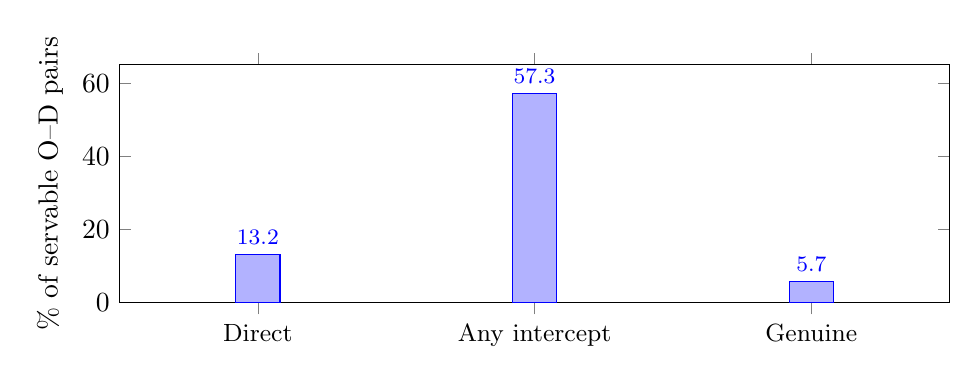
\begin{tikzpicture}
\begin{axis}[
  width=\columnwidth, height=4.6cm,
  ybar, bar width=16pt,
  ymin=0, ymax=65,
  ylabel={\% of servable O--D pairs},
  symbolic x coords={Direct, Any intercept, Genuine},
  xtick=data, x tick label style={font=\small},
  nodes near coords, nodes near coords style={font=\footnotesize},
  enlarge x limits=0.25,
]
\addplot coordinates {(Direct,13.2) (Any intercept,57.3) (Genuine,5.7)};
\end{axis}
\end{tikzpicture}
\caption{Prevalence of itinerary structures. A direct single-route trip is rare
(13.2\%); intercept structures are common (57.3\%).}
\label{fig:prev}
\end{figure}

\subsection{Q2: Frequency advantage}
Among genuine intercepts, the connector-to-target frequency advantage
(Eq.~\ref{eq:adv}) has median $3.1\times$ and mean $3.8\times$; 52.3\% of cases
exceed $3\times$. The median target headway at the junction is 17.9~min against a
median connector headway of 6.0~min near the origin (Table~\ref{tab:head}). This
is the structural reason the maneuver works: riders swap a sparse route for a
frequent one over the first, timing-critical leg.

\begin{table}[t]
\caption{Headways and advantage, genuine-intercept subset (medians).}
\label{tab:head}
\centering
\begin{tabular}{lr}
\toprule
\textbf{Quantity} & \textbf{Value} \\
\midrule
Target headway at junction          & 17.9 min \\
Connector headway near origin       & 6.0 min \\
Frequency advantage $\alpha$ (median) & $3.1\times$ \\
Frequency advantage $\alpha$ (mean)   & $3.8\times$ \\
Share with $\alpha \ge 3\times$       & 52.3\% \\
\bottomrule
\end{tabular}
\end{table}

\subsection{Q3: Reliability model}
For uniformly random passenger arrivals, expected boarding wait is half the
headway, $E[W]=h/2$, and the penalty for mistiming (just missing a vehicle) is a
full headway $h$~\cite{welding1957,larson1981}. Because the intercept rider is
exposed to the \emph{connector's} headway on the timing-critical first leg rather
than the \emph{target's}, we compare $E[W]$ under the two strategies using the
measured median headways. The intercept reduces expected boarding wait from
9.0~min (direct) to 3.0~min, a \textbf{66\% reduction}, and cuts the mistiming
penalty from 17.9~min to 6.0~min (Fig.~\ref{fig:wait}). We emphasize this is a
\emph{reliability} gain, not a scheduled travel-time gain
(Section~\ref{sec:problem}).

\begin{figure}[t]
\centering
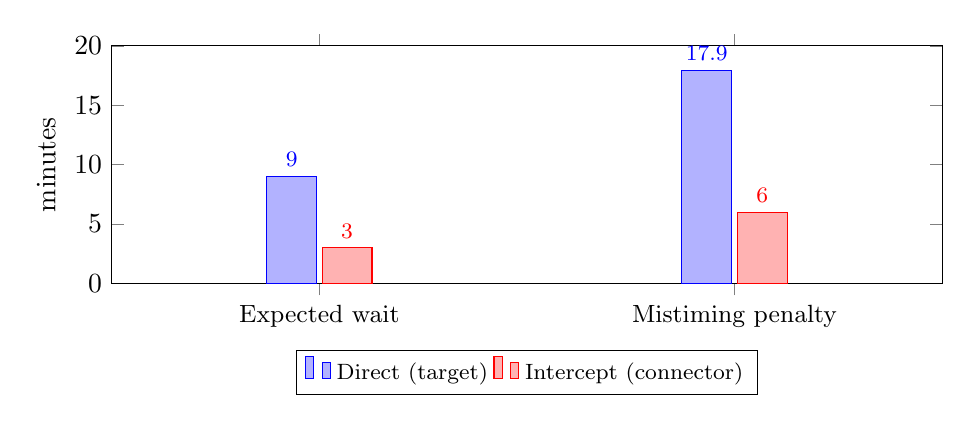
\begin{tikzpicture}
\begin{axis}[
  width=\columnwidth, height=4.6cm,
  ybar, bar width=18pt,
  ymin=0, ymax=20,
  ylabel={minutes},
  symbolic x coords={Expected wait, Mistiming penalty},
  xtick=data, x tick label style={font=\small},
  nodes near coords, nodes near coords style={font=\footnotesize},
  enlarge x limits=0.5,
  legend style={at={(0.5,-0.28)}, anchor=north, legend columns=2, font=\footnotesize},
]
\addplot coordinates {(Expected wait,9.0) (Mistiming penalty,17.9)};
\addplot coordinates {(Expected wait,3.0) (Mistiming penalty,6.0)};
\legend{Direct (target), Intercept (connector)}
\end{axis}
\end{tikzpicture}
\caption{Boarding reliability under the headway model. Riding a frequent
connector over the timing-critical leg cuts expected wait by 66\%.}
\label{fig:wait}
\end{figure}

\subsection{Robustness}
Repeating the batch with a different random seed yields consistent results
(Table~\ref{tab:robust}): direct-route prevalence 13--16\%, intercept-structure
prevalence 57.3\% in both runs, and the key conditional
$P(\text{genuine}\mid\text{direct})$ between 41\% and 43\%. The findings are not
an artifact of a particular sample.

\begin{table}[t]
\caption{Two-seed robustness ($N{=}1500$ each).}
\label{tab:robust}
\centering
\begin{tabular}{lrr}
\toprule
\textbf{Metric} & \textbf{Seed 42} & \textbf{Seed 7} \\
\midrule
Direct prevalence              & 13.2\% & 15.5\% \\
Any intercept structure        & 57.3\% & 57.3\% \\
Genuine intercept              & 5.7\%  & 6.4\% \\
$P(\text{genuine}\mid\text{direct})$ & 43.4\% & 41.2\% \\
Median advantage $\alpha$      & $3.1\times$ & $2.6\times$ \\
\bottomrule
\end{tabular}
\end{table}

\subsection{Case study: a validated real-world intercept}
The project was motivated by a real trip in East Vancouver. The rider travelled
from near Kingsway \& Rupert (postal area V5R~5J9) to the V5S~1Y5 area. The
natural target is route \textbf{\#26}, which runs toward the destination and
passes \textbf{41st~\& Rupert} midway. Both Google Maps and the Transit app
advised walking to a \#26 stop and boarding there. In practice the \#26---already
moving---would be missed on the walk. Instead the rider boarded the
high-frequency \textbf{\#41/R4} nearby, rode to \textbf{41st~\& Rupert}, and
boarded the \emph{same} \#26 downstream, successfully catching it.

Our prototype reconstructs this exactly. It auto-detects the junction (stops
51605~$\leftrightarrow$~51181, 63~m apart), confirms the R4/41 run every
2--4~min at the junction versus the \#26 every $\sim$8--14~min, and---critically---
shows that on \emph{schedule} the direct and intercept boardings catch the same
vehicle (trip 15456609: Earles 08:10 $\rightarrow$ Rupert~\&~41 08:13
$\rightarrow$ Kerr~\&~54 08:18). The maneuver's value is therefore real-time: the
frequent connector lets the rider catch a specific moving bus that walking would
miss. We also observed that not every \#26 trip serves the junction (some early
trips take a different branch), which is exactly why a frequent connector improves
reliability. With the live GTFS-RT feed, the prototype pulled 181 vehicle
positions and 4{,}020 predicted arrivals and correctly evaluated walk-versus-
connector feasibility for the live \#26.

%=======================================================================
\section{Discussion}
\label{sec:discussion}
%=======================================================================
\textbf{Why mainstream planners miss this.} Pareto ranking by (arrival time,
transfers, walking) treats the intercept as a dominated solution: it adds a
boarding without improving scheduled arrival. Our results show that dominance is
an artifact of ignoring reliability and real-time realizability. An
intercept-aware planner can re-admit these itineraries by scoring an extra,
reliability-oriented criterion---e.g.\ exposure to headway on the
timing-critical leg.

\textbf{Schedule vs.\ real time.} The clearest lesson is that the headline
feature---``catch a bus you would otherwise miss''---is fundamentally a real-time
phenomenon. Static analysis establishes that the \emph{opportunity} is common
(Q1--Q3), but only live vehicle positions turn it into a trustworthy ``go now,
you will make it'' instruction. This matches the case study and motivates
treating GTFS-RT as a first-class input rather than an optional enhancement.

\textbf{Practicality.} The entire system is dependency-free and runs the full
regional feed on a laptop, with the batch evaluation completing in under two
seconds. The approach is thus deployable by a single developer and portable to
any GTFS/GTFS-RT agency.

%=======================================================================
\section{Limitations and Threats to Validity}
\label{sec:limits}
%=======================================================================
Our evaluation is structural and schedule-based. (1)~Headways are medians over a
single morning-peak window on one representative weekday; off-peak and weekend
behavior will differ and generally favors intercepts even more (sparser targets).
(2)~We approximate ``what mainstream apps do'' by nearest-stop direct boarding;
we did not instrument the commercial apps directly. (3)~The reliability model
assumes uniform passenger arrivals and uses headway as the exposure proxy; it does
not yet incorporate measured headway \emph{variance} or walking-time uncertainty,
both of which would widen the gap in the intercept's favor. (4)~Representative-trip
stop sequences can under-represent branches; we mitigate this by using the longest
active trip. (5)~The strongest claim---catching specific moving vehicles---was
validated on one real trip and in live feed pulls, not yet in a large real-time
field study. Addressing (5) is the central item of future work.

%=======================================================================
\section{Future Work}
%=======================================================================
We plan a longitudinal real-time study: log, across many O--D pairs and times of
day, how often an intercept catches a target that walking provably could not, and
by how much. This yields the definitive empirical claim the static analysis can
only motivate. We also intend to (i)~integrate the intercept criterion into a
full engine such as OpenTripPlanner~\cite{otp} as a re-ranking layer,
(ii)~replace nearest-stop baselines with the actual itineraries returned by
commercial planners for a head-to-head comparison, (iii)~incorporate
headway-variance and walk-time distributions into the reliability model, and
(iv)~add address geocoding and a mobile (PWA/native) client for field use.

%=======================================================================
\section{Conclusion}
%=======================================================================
Experienced transit riders know a trick that trip planners do not show: ride a
frequent connector to a downstream junction and board the target bus there. We
formalized this chase-and-intercept structure, built a transparent prototype over
the full live Metro Vancouver feed that discovers intercept junctions
automatically, and measured the phenomenon. Intercept structures are common
(57.3\% of servable O--D pairs), and when a direct route exists a more-frequent
connector intercept is \emph{also} available 43.4\% of the time, cutting expected
boarding wait by 66\% under a standard headway model. A validated real trip shows
why the feature's full power is realized with real-time data. Intercept routing is
common, well-defined, and worth surfacing---and standard planners are leaving it
on the table.

%=======================================================================
\section*{Reproducibility}
%=======================================================================
The planner, automatic junction detector, real-time evaluator, and the evaluation
harness (\texttt{src/evaluate.js}, which emits the per-pair CSV and all summary
statistics reported here) are released with the project. All numbers in
Section~\ref{sec:eval} are regenerated by
\texttt{node src/evaluate.js 1500 20261007 42}.

\bibliographystyle{IEEEtran}
\bibliography{refs}

\end{document}
